\documentclass[11pt,a4paper]{ctexart}
\usepackage[student]{../../../common/ipara}
\tcbuselibrary{breakable}
\usepackage{tikz-3dplot}

% =====================================================
% 题型：立体几何解答题 / 折叠与最值问题 (q_solid_folding_rectangle.tex)
% =====================================================
% =====================================================
% 难度：★★★ (难题)
% =====================================================
\newcommand{\qSolidFoldingRectangleStem}{%
  如图，在矩形 $ABCD$ 中，$AB=1$，$BC=\sqrt{3}$，$M$ 是线段 $AD$ 上的一动点，将 $\triangle ABM$ 沿着 $BM$ 折起，使点 $A$ 到达点 $A'$ 的位置，满足点 $A' \notin$ 平面 $BCDM$，且点 $A'$ 在平面 $BCDM$ 内的射影 $E$ 落在线段 $BC$ 上。
  \begin{enumerate}[label=(\arabic*), leftmargin=2em, itemsep=0.1em]
    \item 当点 $M$ 与端点 $D$ 重合时，证明：$A'B \perp$ 平面 $A'CD$；
    \item 当 $AM=\dfrac{3}{2}$ 时，求二面角 $A'-BM-C$ 的余弦值；
    \item 设直线 $CD$ 与平面 $A'BM$ 所成的角为 $\alpha$，二面角 $A'-BM-C$ 的平面角为 $\beta$，求 $\sin^2\alpha \cos\beta$ 的最大值。
  \end{enumerate}%
}

\newcommand{\qSolidFoldingRectangleFigure}[1][1.0]{%
  \begin{tikzpicture}[scale=#1, >=stealth, line join=round, line cap=round]
    % 左图：折叠前
    \begin{scope}[xshift=0cm, yshift=0cm]
      % 定义顶点
      \coordinate (B) at (0, 0);
      \coordinate (C) at (2.6, 0);
      \coordinate (D) at (2.6, 1.5);
      \coordinate (A) at (0, 1.5);
      \coordinate (M) at (1.8, 1.5);
      \coordinate (E) at (1.25, 0);
      \coordinate (F) at (0.74, 0.62);
      
      % 绘制矩形和折痕
      \draw[thick] (A) -- (B) -- (C) -- (D) -- cycle;
      \draw[thick, dashed, blue] (B) -- (M);
      \draw[thick, dashed, red] (A) -- (E);
      
      % 标记点
      \fill (A) circle (1.2pt) node[above left] {\small $A$};
      \fill (B) circle (1.2pt) node[below left] {\small $B$};
      \fill (C) circle (1.2pt) node[below right] {\small $C$};
      \fill (D) circle (1.2pt) node[above right] {\small $D$};
      \fill (M) circle (1.2pt) node[above] {\small $M$};
      \fill (E) circle (1.2pt) node[below] {\small $E$};
      \fill (F) circle (1.2pt) node[above left] {\small $F$};
      
      % 直角标记
      \draw[gray, thin] ($(F)!0.1!(A)$) -- ($($(F)!0.1!(A)$) + ($(F)!0.1!(M)$) - (F)$) -- ($(F)!0.1!(M)$);
      
      \node[below] at (1.3, -0.2) {\small 折叠前};
    \end{scope}
    
    % 折叠箭头
    \draw[->, very thick, gray] (3.0, 0.75) -- (4.0, 0.75) node[midway, above] {\small 折叠};
    
    % 右图：折叠后
    \begin{scope}[xshift=4.5cm, yshift=0cm]
      % 定义顶点 (精确计算的投影三维坐标)
      \coordinate (B) at (0, 0);
      \coordinate (C) at (2.6, 0);
      \coordinate (D) at (3.2, 0.9);
      \coordinate (M) at (2.55, 0.9);
      \coordinate (E) at (1.15, 0);
      \coordinate (A1) at (1.15, 0.96);
      \coordinate (F) at (1.02, 0.36); % BM 上的垂足 F
      
      % 绘制底面边界与棱
      \draw[thick] (B) -- (C) -- (D);
      \draw[thick, dashed, gray!60] (D) -- (M);
      \draw[thick, dashed, gray!60] (M) -- (B);
      
      % 绘制折起后的面 A'BM 和 A'BC
      \draw[thick, blue] (A1) -- (B);
      \draw[thick, blue] (A1) -- (M);
      \draw[thick] (A1) -- (C);
      \draw[thick, dashed, gray!60] (A1) -- (D);
      
      % 绘制辅助线
      \draw[thick, dashed, red] (A1) -- (E);
      \draw[thick, dashed, red] (E) -- (F);
      \draw[thick, dashed, red] (A1) -- (F);
      
      % 标记点
      \fill (B) circle (1.2pt) node[below left] {\small $B$};
      \fill (C) circle (1.2pt) node[below right] {\small $C$};
      \fill (D) circle (1.2pt) node[above right] {\small $D$};
      \fill (M) circle (1.2pt) node[above right] {\small $M$};
      \fill (E) circle (1.2pt) node[below] {\small $E$};
      \fill (A1) circle (1.2pt) node[above] {\small $A'$};
      \fill (F) circle (1.2pt) node[left] {\small $F$};
      
      % 直角标记
      % A'E \perp base
      \draw[red, thin] ($(E)!0.08!(A1)$) -- ($($(E)!0.08!(A1)$) + ($(E)!0.08!(B)$) - (E)$) -- ($(E)!0.08!(B)$);
      % A'F \perp BM
      \draw[red, thin] ($(F)!0.08!(A1)$) -- ($($(F)!0.08!(A1)$) + ($(F)!0.08!(M)$) - (F)$) -- ($(F)!0.08!(M)$);
      % EF \perp BM
      \draw[red, thin] ($(F)!0.08!(E)$) -- ($($(F)!0.08!(E)$) + ($(F)!0.08!(M)$) - (F)$) -- ($(F)!0.08!(M)$);
      
      \node[below] at (1.3, -0.2) {\small 折叠后};
    \end{scope}
  \end{tikzpicture}%
}

\newcommand{\qSolidFoldingRectangleAnswer}{%
  (1) 证明见解析；(2) 二面角 $A'-BM-C$ 的余弦值为 $\dfrac{4}{9}$；(3) $\sin^2\alpha \cos\beta$ 的最大值为 $\dfrac{1}{4}$.%
}

\newcommand{\qSolidFoldingRectangleSolution}{%
  【解题思路】\\
  本题为折叠几何综合最值难题。解题的关键在于抓住折叠前后的“距离与角度不变性”，通过代数建模构建起动态线段的长度关系网络：
  \begin{enumerate}[label=\arabic*.]
    \item \textbf{建立核心长度模型}：设 $AM=x$。通过 $A'$ 在底面的射影 $E$ 落在 $BC$ 上这一临界条件，结合折叠前后 $A'B=AB=1, A'M=AM=x$ 及 $A'E \perp$ 平面 $BCDM$，在底面利用 Rt$\triangle A'EB$ 和 Rt$\triangle A'EM$ 构建方程，推导得出 $BE = \dfrac{1}{x}$，此式为全题的计算发动机。
    \item \textbf{几何垂直证明}：当 $M=D$ 时，长度参数 $x=\sqrt{3}$ 确定。利用勾股定理逆定理在 $\triangle A'BC$ 中求证 $A'B \perp A'C$，再利用线面垂直定理证明 $CD \perp$ 平面 $A'BC$ 从而得到 $CD \perp A'B$，最终证明 $A'B \perp$ 平面 $A'CD$。
    \item \textbf{二面角计算}：利用三垂线定理判定二面角 $A'-BM-C$ 的平面角为 $\angle A'FE$。通过底面三角形面积法计算出 $EF$，再结合折叠前后 $A'F=AF$（即 $A$ 到折痕 $BM$ 的距离），在直角三角形 $\triangle A'EF$ 中直接求出 $\cos\beta = \dfrac{EF}{A'F} = \dfrac{1}{x^2}$。
    \item \textbf{最值求解与三正弦定理模型识别}：注意到直线 $CD$ 在底面内，平面 $A'BM$ 是底面绕 $BM$ 折起形成的。根据\textbf{三正弦定理（最大角定理）}，直线与折起平面所成的角 $\alpha$、折起二面角 $\beta$ 以及直线与折痕的夹角 $\theta$ 满足：$\sin\alpha = \sin\beta \sin\theta$。由此将线面角转化为关于 $x$ 的代数式，化简后应用二次函数求最值。
  \end{enumerate}

  【解析计算】\\
  \noindent\textbf{核心关系推导：}\\
  设 $AM=x$，$A'$ 在底面上的射影为 $E \in BC$，则 $A'E \perp$ 平面 $BCDM$。\\
  因为折叠是绕 $BM$ 进行的刚体旋转，折叠前后距离保持不变，故有：
  \[ A'B = AB = 1,\quad A'M = AM = x \]
  由于 $A'E \perp$ 平面 $BCDM$，且 $B, C, E \subset$ 平面 $BCDM$，所以 $A'E \perp BC$。\\
  在 Rt$\triangle A'EB$ 中，有：
  \[ A'E^2 = A'B^2 - BE^2 = 1 - BE^2 \quad \text{—— 方程 (1)} \]
  在底面矩形中，过 $M$ 作 $MM_0 \perp BC$ 于 $M_0$，由矩形性质可知 $BM_0 = AM = x, MM_0 = AB = 1$。\\
  由于 $E \in BC$，在 Rt$\triangle EM_0M$ 中，有：
  \[ EM^2 = EM_0^2 + MM_0^2 = (BE - x)^2 + 1 \]
  在 Rt$\triangle A'EM$ 中，因为 $A'E \perp$ 平面 $BCDM$，所以 $A'E \perp EM$。则有：
  \[ A'M^2 = EM^2 + A'E^2 \implies x^2 = (BE - x)^2 + 1 + A'E^2 \quad \text{—— 方程 (2)} \]
  将方程 (1) 代入方程 (2)，消去 $A'E^2$ 得：
  \[ x^2 = (BE - x)^2 + 1 + (1 - BE^2) \]
  展开整理得：
  \[ x^2 = BE^2 - 2x \cdot BE + x^2 + 2 - BE^2 \implies 2x \cdot BE = 2 \implies \boxed{BE = \frac{1}{x}} \]
  代入方程 (1) 中，可得 $A'$ 的投影高度为：
  \[ \boxed{A'E = \sqrt{1 - \frac{1}{x^2}}} \]
  要使折起后的几何体存在，高 $A'E$ 必须为实数且不为 $0$，即 $1 - \frac{1}{x^2} > 0 \implies x > 1$。\\
  又因为点 $M$ 在线段 $AD$ 上，且 $AD = \sqrt{3}$，所以 $x \le \sqrt{3}$。\\
  故动点参数 $x$ 的取值范围为 $\boxed{x \in [1, \sqrt{3}]}$。

  \noindent\textbf{（1）证明：当 $M=D$ 时，$A'B \perp$ 平面 $A'CD$}\\
  当点 $M$ 与端点 $D$ 重合时，其长度参数 $x = AM = AD = BC = \sqrt{3}$。\\
  此时可得：
  \[ BE = \frac{1}{\sqrt{3}},\quad CE = BC - BE = \sqrt{3} - \frac{1}{\sqrt{3}} = \frac{2}{\sqrt{3}} \]
  高度的平方为：
  \[ A'E^2 = 1 - \frac{1}{x^2} = 1 - \frac{1}{3} = \frac{2}{3} \]
  在 Rt$\triangle A'EC$ 中，有：
  \[ A'C^2 = A'E^2 + CE^2 = \frac{2}{3} + \left(\frac{2}{\sqrt{3}}\right)^2 = \frac{2}{3} + \frac{4}{3} = 2 \]
  在 $\triangle A'BC$ 中，因为 $A'B = 1, BC = \sqrt{3}$，且 $A'C = \sqrt{2}$。\\
  易见：
  \[ A'B^2 + A'C^2 = 1^2 + (\sqrt{2})^2 = 3 = BC^2 \]
  根据勾股定理逆定理，可知 $\boxed{A'B \perp A'C}$。\\
  在底面矩形中，$CD \perp BC$。又因为 $A'E \perp$ 平面 $BCDM$，且 $CD \subset$ 平面 $BCDM$，所以 $CD \perp A'E$。\\
  由于 $BC \cap A'E = E$，所以 $CD \perp$ 平面 $A'BC$。\\
  因为 $A'B \subset$ 平面 $A'BC$，所以有 $\boxed{CD \perp A'B}$。\\
  由于 $A'C \cap CD = C$，且 $A'C, CD \subset$ 平面 $A'CD$，\\
  综上所述，$A'B$ 垂直于平面 $A'CD$ 内的两条相交直线，故有：
  \[ \boxed{A'B \perp \text{平面 } A'CD} \]

  \noindent\textbf{（2）求解二面角 $A'-BM-C$ 的平面角：}\\
  在底面内，过点 $E$ 作 $EF \perp BM$ 于点 $F$，连接 $A'F$。\\
  因为 $A'E \perp$ 平面 $BCDM$，且 $EF \perp BM$，根据三垂线定理可知，$\boxed{A'F \perp BM}$。\\
  因此，$\angle A'FE$ 即为二面角 $A'-BM-C$ 的平面角 $\beta$。\\
  在直角三角形 $\triangle ABM$ 中，斜边为 $BM = \sqrt{AM^2 + AB^2} = \sqrt{x^2 + 1}$。\\
  在底面中，三角形 $\triangle BEM$ 的面积可以表示为：
  \[ S_{\triangle BEM} = \frac{1}{2} \cdot BE \cdot AB = \frac{1}{2} \cdot \frac{1}{x} \cdot 1 = \frac{1}{2x} \]
  同时，以 $BM$ 为底，高为 $EF$，其面积也可以表示为：
  \[ S_{\triangle BEM} = \frac{1}{2} \cdot BM \cdot EF = \frac{1}{2} \cdot \sqrt{x^2+1} \cdot EF \]
  联立面积公式，求得 $EF$ 的长度为：
  \[ EF = \frac{1}{x\sqrt{x^2+1}} \]
  折叠前，点 $A$ 到折痕 $BM$ 的距离等于折起后点 $A'$ 到折痕 $BM$ 的距离（即 $A'F$）。\\
  在直角三角形 $\triangle ABM$ 中，由等面积法有：
  \[ S_{\triangle ABM} = \frac{1}{2} \cdot AB \cdot AM = \frac{x}{2} = \frac{1}{2} \cdot BM \cdot A'F \implies A'F = \frac{x}{\sqrt{x^2+1}} \]
  在 Rt$\triangle A'EF$ 中，二面角 $\beta = \angle A'FE$ 的余弦值为：
  \[ \cos\beta = \frac{EF}{A'F} = \frac{\frac{1}{x\sqrt{x^2+1}}}{\frac{x}{\sqrt{x^2+1}}} = \boxed{\frac{1}{x^2}} \]
  当 $AM = \frac{3}{2}$ 即 $x = \frac{3}{2}$ 时，代入可得：
  \[ \cos\beta = \frac{1}{\left(\frac{3}{2}\right)^2} = \frac{4}{9} \]
  故所求二面角 $A'-BM-C$ 的余弦值为 $\boxed{\dfrac{4}{9}}$。

  \noindent\textbf{（3）求 $\sin^2\alpha \cos\beta$ 的最大值：}\\
  在底面矩形中，直线 $CD \parallel AB$，所以直线 $CD$ 与折痕 $BM$ 所成的角 $\theta$ 等于直线 $AB$ 与 $BM$ 所成的角。\\
  在直角三角形 $\triangle ABM$ 中，有：
  \[ \sin\theta = \frac{AM}{BM} = \frac{x}{\sqrt{x^2+1}} \]
  直线 $CD$ 位于底面内，平面 $A'BM$ 是由底面的一部分绕 $BM$ 折起形成的，且这两个平面的夹角为 $\beta$。\\
  根据\textbf{三正弦定理（最大角定理）}，直线 $CD$ 与平面 $A'BM$ 所成的线面角 $\alpha$ 满足关系式：
  \[ \sin\alpha = \sin\beta \sin\theta \]
  由（2）中求得 $\cos\beta = \frac{1}{x^2}$，由于 $x \in [1, \sqrt{3}]$，故有：
  \[ \sin\beta = \sqrt{1 - \cos^2\beta} = \sqrt{1 - \frac{1}{x^4}} \]
  代入可求得：
  \[ \sin^2\alpha = \sin^2\beta \sin^2\theta = \left(1 - \frac{1}{x^4}\right) \cdot \frac{x^2}{x^2+1} = \frac{x^4-1}{x^4} \cdot \frac{x^2}{x^2+1} \]
  利用平方差公式进行化简：
  \[ \sin^2\alpha = \frac{(x^2-1)(x^2+1)}{x^4} \cdot \frac{x^2}{x^2+1} = \frac{x^2-1}{x^2} \]
  由此可得目标代数式为：
  \[ \sin^2\alpha \cos\beta = \frac{x^2-1}{x^2} \cdot \frac{1}{x^2} = \frac{x^2-1}{x^4} \]
  令 $t = x^2$。因为 $x \in [1, \sqrt{3}]$，所以 $t \in [1, 3]$。\\
  则代数式化为：
  \[ f(t) = \frac{t-1}{t^2} = \frac{1}{t} - \frac{1}{t^2} \]
  进一步令 $u = \frac{1}{t}$。因为 $t \in [1, 3]$，所以 $u \in \left[\frac{1}{3}, 1\right]$。\\
  目标二次函数为：
  \[ g(u) = u - u^2 = -\left(u - \frac{1}{2}\right)^2 + \frac{1}{4} \]
  因为对称轴 $u = \frac{1}{2} \in \left[\frac{1}{3}, 1\right]$，所以当 $u = \frac{1}{2}$（即 $t = 2 \implies x = \sqrt{2} \in [1, \sqrt{3}]$）时，函数取得最大值，最大值为：
  \[ g\left(\frac{1}{2}\right) = \frac{1}{4} \]
  故所求 $\sin^2\alpha \cos\beta$ 的最大值为 $\boxed{\dfrac{1}{4}}$。
}

\newcommand{\qSolidFoldingRectangleDiagnosis}{%
  用于课堂精准提优训练。本题是一道非常经典的矩形折叠最值难题。重点考查折叠前后“长度与角度的守恒性”以及将动态几何特征转化为代数方程的能力。在解析中应引导学生识别出“三正弦定理”在求线面角最值中的应用，免去在折叠后的复杂空间体系中寻找线面角投影的繁琐作图过程。
}

\newcommand{\qSolidFoldingRectangleTeachingNotes}{%
  \item \textbf{教学核心与模型识别提示}：
    \begin{itemize}
      \item \textbf{折叠动力引擎}：引导学生先建立折起高 $A'E = \sqrt{1 - \frac{1}{x^2}}$ 与投影点位置 $BE = \frac{1}{x}$ 的代数关系，这是折叠模型中利用垂直平分性质建立等式的一个非常典型的“保距消元”手法，务必让学生彻底掌握这一推导。
      \item \textbf{三正弦定理的妙用}：第（3）问中，如果按照常规思路去寻找直线 $CD$ 在平面 $A'BM$ 上的投影来求线面角 $\alpha$，空间想象难度极大且极易出错。这里直接把底面看作平面 $\beta$，平面 $A'BM$ 看作平面 $\alpha$，直线 $CD$ 位于底面内，利用\textbf{三正弦定理} $\sin\alpha = \sin\beta \sin\theta$（线面角正弦 = 二面角正弦 $\times$ 面内线与交线夹角正弦），直接跳过了复杂的空间垂足寻找过程，是极佳的模型识别实战案例。
    \end{itemize}
}


\renewcommand{\studentthink}[1]{%
  \vspace{0.4em}
  {\small\textbf{思考与自查：}}
  \begin{enumerate}[label=\arabic*. , leftmargin=2em, itemsep=0.15em, topsep=0.2em]
    #1
  \end{enumerate}
}

% =====================================================
% 学案公式三线表定义
% =====================================================
\newcommand{\formulatable}{%
  \arrayrulecolor{rulecolor}% 设置表格内划线颜色
  \begin{tabularx}{\textwidth}{p{3.8cm}X}
  \toprule[1.2pt]
  线面垂直判定 & 若一条直线垂直于平面内的两条 \fblank[2cm]{相交} 直线，则这条直线垂直于该平面。\\ \hline
  面面垂直判定 & 若一个平面内有一条直线垂直于另一个平面，则这两个平面 \fblank[2cm]{垂直}。\\ \hline
  线面角定义 & 直线与平面所成角，是这条直线与它在该平面内的 \fblank[2.5cm]{射影} 所成的角。\\ \hline
  线面角正弦公式 & 设斜线长为 $l$，斜线端点到平面的距离为 $h$，则线面角 $\theta$ 满足 \(\sin\theta = \fblank[2.5cm]{\displaystyle\frac{h}{l}}\)。\\ \hline
  三棱锥体积公式 & \(V = \fblank[3.5cm]{\displaystyle\frac{1}{3} S_{\text{底}} h_{\text{高}}}\) \\ \hline
  三余弦定理公式 & 设斜线与平面的线面角为 $\theta$，斜影与平面内直线的夹角为 $\beta$，斜线与该直线的夹角为 $\gamma$，则有 \(\cos\gamma = \fblank[3.5cm]{\cos\theta \cos\beta}\)。\\ \hline
  三正弦定理公式 & 设斜面与底面的二面角为 $\varphi$，斜线与二面角棱的夹角为 $\theta_1$，斜线与底面所成线面角为 $\theta_2$，则有 \(\sin\theta_2 = \fblank[3.5cm]{\sin\varphi \sin\theta_1}\)。\\ \hline
  三射线定理公式 & 设三条射线两两夹角为 $\alpha, \beta, \gamma$，其所对的二面角为 $\varphi_1$，则二面角的余弦值为 \(\cos\varphi_1 = \fblank[4.5cm]{\displaystyle\frac{\cos\alpha - \cos\beta\cos\gamma}{\sin\beta\sin\gamma}}\)。\\ \hline
  余弦定理 (边角关系) & 在 \(\triangle ABC\) 中，\(\cos C = \fblank[4.5cm]{\displaystyle\frac{a^2+b^2-c^2}{2ab}}\) （用三边表示）。\\ \hline
  三角形面积公式 & 在 \(\triangle ABC\) 中，已知角 $C$ 及其夹边 $a, b$，则面积 \(S = \fblank[4.5cm]{\displaystyle\frac{1}{2}ab\sin C}\)。\\
  \bottomrule[1.2pt]
  \end{tabularx}%
}

% =====================================================
% 页眉页脚设置
% =====================================================
\pagestyle{fancy}
\fancyhf{}
\lhead{\small 立体几何专题学案}
\rhead{\small 专题：空间线段与极值计算}
\cfoot{\small 第 \thepage\ 页\quad 共 \pageref{LastPage} 页}
\renewcommand{\headrulewidth}{0.4pt}
\renewcommand{\footrulewidth}{0pt}

\begin{document}

% =====================================================
% 第一页：课前公式复习
% =====================================================
\begin{center}
  {\Large\bfseries 立体几何专题学案：空间线段与极值计算}\\
  \vspace{0.6em}
  姓名：\blank{3cm}
  \quad
  班级：\blank{3cm}
  \quad
  日期：\blank{3cm}
\end{center}

\section{课前公式复习}
\begin{tcolorbox}[colback=black!2, colframe=black!40, title=复习指南, arc=2pt]
  空间角的计算与极值分析是高考立体几何的压轴难点。在动笔前，请务必熟练掌握以下核心公式。
\end{tcolorbox}

\begingroup
\large
\renewcommand{\arraystretch}{1.6}
\linespread{1.5}\selectfont
\showprompttrue 
\formulatable
\endgroup

\newpage

% =====================================================
% 第二页：核心定理与小试身手
% =====================================================
\section{四大核心定理小试身手}

\begin{tcolorbox}[colback=black!1, colframe=black!30, size=small]
  利用空间角的四大定理（三余弦、三正弦、三夹角、三射线）可以绕开复杂的建系和几何找垂线过程，快速实现空间角的转化。
\end{tcolorbox}

\problemheader{小试身手 1（两个斜角求三棱柱的高）}
设斜三棱柱中，侧棱 $CC_1 = 1$，底面满足 $\angle ACB = 90^\circ$。已知侧棱与底面边缘的夹角满足 $\angle ACC_1 = 60^\circ, \angle BCC_1 = 45^\circ$。求三棱柱的高。
\choiceworkarea[4.8cm]

\problemheader{小试身手 2（利用对称性确定投影方向）}
在斜三棱柱中，底面满足 $AB = AC = 1, \angle BAC = 90^\circ$。侧棱满足 $AA_1 = 2$，且侧棱与底面两边的夹角相等，均为 $\angle A_1AB = \angle A_1AC = 60^\circ$。求对应四面体 $A_1-ABC$ 的体积。
\choiceworkarea[4.8cm]

\problemheader{小试身手 3（等边底面中的线面角）}
若底面为等边三角形 $ABC$，侧棱 $AA_1$ 与底面内相邻两边 $AB, AC$ 的夹角均为 $45^\circ$。求侧棱 $AA_1$ 与底面所成的线面角 $\theta$ 的余弦值。
\choiceworkarea[3.6cm]

\newpage

% =====================================================
% 第三页：深度探究题一（斜四棱柱计算）
% =====================================================
\section{课堂深度探究题}

\problemheader{探究一：斜四棱柱中的线段与距离计算}
已知在四棱柱 $ABCD-A_1B_1C_1D_1$ 中，四边形 $ABCD$ 为菱形，$AA_1 = AC_1 = AB = 2$，$\angle BAD = 60^\circ$，$\angle AA_1B_1 = \angle AA_1D_1$，$E$ 是侧棱 $CC_1$ 上的一点。

\begin{center}
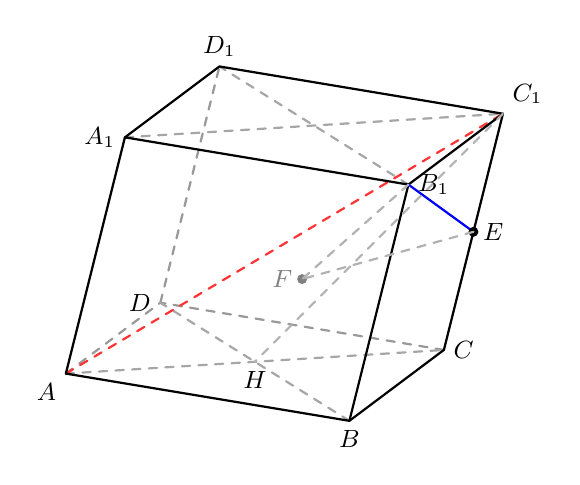
\begin{tikzpicture}[scale=1.5, >=stealth, line join=round, line cap=round]
    % 顶点坐标
    \coordinate (A) at (0,0);
    \coordinate (B) at (2.4,-0.4);
    \coordinate (D) at (0.8,0.6);
    \coordinate (C) at (3.2,0.2);
    
    \coordinate (A1) at (0.5,2.0);
    \coordinate (B1) at (2.9,1.6);
    \coordinate (D1) at (1.3,2.6);
    \coordinate (C1) at (3.7,2.2);
    
    \coordinate (E) at ($(C1)!0.5!(C)$); % 侧棱 CC1 上的点 E
    
    % 隐藏线（背面）
    \draw[dashed, thick, gray!80] (A) -- (D);
    \draw[dashed, thick, gray!80] (C) -- (D);
    \draw[dashed, thick, gray!80] (D) -- (D1);
    \draw[dashed, thick, gray!70] (A) -- (C);
    \draw[dashed, thick, gray!70] (B) -- (D);
    \draw[dashed, thick, gray!70] (A1) -- (C1);
    \draw[dashed, thick, gray!70] (B1) -- (D1);
    \draw[dashed, thick, red!80] (A) -- (C1);
    
    % 可见实线
    \draw[thick] (A) -- (B) -- (C) -- (C1) -- (D1) -- (A1) -- cycle;
    \draw[thick] (B) -- (B1) -- (C1);
    \draw[thick] (A1) -- (B1);
    \draw[thick, blue] (B1) -- (E);
    
    \fill (E) circle (1.2pt) node[right] {\small $E$};
    
    % 辅助讲解线：垂线
    \coordinate (H) at (1.6,0.1); % AC 中点 H
    \draw[dashed, thick, gray!60] (C1) -- (H);
    \node[below] at (H) {\small $H$};
    
    \coordinate (E0) at (2.0,0.8);
    \fill[gray] (E0) circle (1.2pt) node[left] {\small $F$};
    \draw[dashed, thick, gray!60] (E) -- (E0);
    \draw[dashed, thick, gray!60] (B1) -- (E0);
    
    \node[below left] at (A) {\small $A$};
    \node[below] at (B) {\small $B$};
    \node[right] at (C) {\small $C$};
    \node[left] at (D) {\small $D$};
    \node[left] at (A1) {\small $A_1$};
    \node[right] at (B1) {\small $B_1$};
    \node[above right] at (C1) {\small $C_1$};
    \node[above] at (D1) {\small $D_1$};
\end{tikzpicture}
\end{center}

\subsection*{第（1）问：证明 $AA_1 \perp B_1D_1$}
\answerblank[6.2cm]{证明：}
\studentthink{
  \item 要证明线线垂直，我们可以利用面面垂直，或者线面垂直。本题中两条直线是异面直线，你打算把哪一条线放入哪一个平面，再证明另一条线垂直该平面？
  \item $\triangle AA_1B_1$ 与 $\triangle AA_1D_1$ 全等的已知条件是什么？这能推出什么相等的线段？
}

\newpage

% =====================================================
% 第四页：深度探究题一第（2）、（3）问
% =====================================================
\subsection*{第（2）问：求点 $E$ 到平面 $AA_1B_1B$ 的距离}
\answerblank[7.2cm]{解：}

\subsection*{第（3）问：若直线 $B_1E$ 与平面 $AA_1B_1B$ 所成角的正弦值为 $\dfrac{\sqrt{42}}{14}$，求 $C_1E$ 的长度}
\answerblank[9.8cm]{解：}
\studentthink{
  \item 第（2）问中求点到平面的距离，是否可以直接利用体积极值或投影法？点 $E$ 在侧棱 $CC_1$ 上，它到侧面 $AA_1B_1B$ 的距离与 $C_1$ 到该平面的距离有什么关系？
  \item 第（3）问中，直线上某点到平面的垂足为 $F$，则直线上任一点与垂足的连线与平面所成的角即为线面角。本问的线面角正弦值与斜线 $B_1E$、垂线段有什么数量关系？
}

\newpage

% =====================================================
% 第五页：深度探究题二（体积极值问题）
% =====================================================
\problemheader{探究二：三棱锥体积极值问题}
已知三棱锥 $P-ABC$ 的底面是边长为 3 的正三角形，点 $A$ 在侧面 $PBC$ 上的射影 $G$ 是 $\triangle PBC$ 的垂心，且点 $G$ 不在 $\triangle PBC$ 的外部。当三棱锥体积最小时，$PA$ 的长是多少？

\begin{center}
\tdplotsetmaincoords{70}{105} 
\begin{tikzpicture}[tdplot_main_coords, scale=2.2, line join=round, line cap=round]
    % 三维坐标系：底面正三角形中心置于原点，A 点朝向正前方
    \coordinate (A) at (0, {-sqrt(3)}, 0);
    \coordinate (B) at (1.5, {sqrt(3)/2}, 0);
    \coordinate (C) at (-1.5, {sqrt(3)/2}, 0);
    \coordinate (O) at (0,0,0);
    
    % 高度设定
    \def\h{2.2} 
    \coordinate (P) at (0, 0, \h);
    
    % BC 中点 M
    \coordinate (M) at (0, {sqrt(3)/2}, 0);
    
    % 垂心 G
    \def\t{0.5975}
    \coordinate (G) at (0, {\t*sqrt(3)/2}, {\h*(1-\t)});

    % 底层结构 (虚线)
    \draw[dashed, thick, black!60] (C) -- (A);
    \draw[dashed, thick, black!60] (A) -- (B);
    \draw[dashed, thick, black!50] (A) -- (O);
    \draw[dashed, thick, black!50] (P) -- (O);
    \draw[dashed, blue, thick, opacity=0.7] (A) -- (M);

    % 后方侧面 PBC (半透明蒙版)
    \filldraw[fill=cyan!8, opacity=0.9, thick] (P) -- (B) -- (C) -- cycle;

    % 前端侧棱
    \draw[thick] (P) -- (A);
    \draw[blue, thick] (P) -- (M); 

    % 核心投影线 (红色加粗)
    \draw[dashed, red, thick] (A) -- (G);

    % 空间直角标记
    \coordinate (G1) at ($(G)!0.15cm!(A)$);
    \coordinate (G2) at ($(G)!0.15cm!(M)$);
    \coordinate (G3) at ($(G1)+(G2)-(G)$);
    \draw[red, thick] (G1) -- (G3) -- (G2);

    % 标注
    \node[below, shift={(0,-0.1)}] at (A) {$A$};
    \node[right, shift={(0.1,0)}] at (B) {$B$};
    \node[left, shift={(-0.1,0)}] at (C) {$C$};
    \node[above, shift={(0,0.1)}] at (P) {$P$};
    \node[below right, shift={(0.05,-0.05)}] at (O) {$O$};
    \node[below right, shift={(0.05,-0.05)}] at (M) {$M$};
    \node[above right, red, shift={(0.05,0.05)}] at (G) {$G$};
\end{tikzpicture}
\end{center}

\answergrid[10.5cm]{解：}
\postproblem{
  \item 第一步，先证明三棱锥 $P-ABC$ 是正三棱锥（利用射影垂直关系与对棱垂直的性质）；
  \item 第二步，挖掘“垂心不在三角形外部”的临界条件。由侧面为等腰三角形，顶角 $\angle BPC$ 的限制是什么？
  \item 第三步，写出高 $PO$ 与侧棱 $PA$ 的代数函数关系式，利用余弦定理建立关于侧棱长的范围，求出最小值。
}{
  \checkbox 证明了 $P-ABC$ 是正三棱锥 \quad
  \checkbox 找出了 $\angle BPC \le 90^\circ$ 的临界限制 \quad
  \checkbox 结合余弦定理求得了侧棱长的最小值
}{1.6cm}

\newpage

% =====================================================
% 探究三：折叠最值综合探究
% =====================================================
\problemheader{探究三：矩形折叠与最值问题（综合实战）}
\qSolidFoldingRectangleStem

\begin{center}
  \qSolidFoldingRectangleFigure[1.2]
\end{center}

\subsection*{第（1）问：当点 $M$ 与端点 $D$ 重合时，证明 $A'B \perp$ 平面 $A'CD$}
\answerblank[5.8cm]{证明：}

\newpage
\subsection*{第（2）问：当 $AM=\dfrac{3}{2}$ 时，求二面角 $A'-BM-C$ 的余弦值}
\answerblank[6.8cm]{解：}

\subsection*{第（3）问：求 $\sin^2\alpha \cos\beta$ 的最大值}
\answerblank[7.8cm]{解：}
\postproblem{
  \item 抓住折叠前后的“保距与保角性”。折起后哪些线段长度没有改变？
  \item 第（2）问中，如何运用面积法计算 $EF$ 的长度？点 $A'$ 到折痕 $BM$ 的距离折前折后是如何守恒的？
  \item 第（3）问中，折起面与底面的交线是 $BM$。你能否识别出直线 $CD$ 与折起面夹角 $\alpha$、二面角 $\beta$、面内线与交线夹角 $\theta$ 的“三正弦定理”关系：$\sin\alpha = \sin\beta\sin\theta$？这能帮你省去多少建系或作图的计算？
}{
  \checkbox 建立了折叠模型的核心长度代数式 $BE = \frac{1}{x}$ \quad
  \checkbox 找准了二面角平面角 $\angle A'FE$ 并完成了计算 \quad
  \checkbox 识别并应用了三正弦定理模型求最值
}{1.6cm}

\newpage

% =====================================================
% 第六页：学习总结与自查
% =====================================================
\begin{center}
  {\Large\bfseries 学习总结与公式默写}
\end{center}

\setcounter{section}{0} % 重置第一级标题编号，重新从“一”开始

\section{公式二次默写}
\begingroup
\large
\renewcommand{\arraystretch}{1.6}
\linespread{1.5}\selectfont
\showpromptfalse 
\formulatable
\endgroup

\section{本专题核心方法与易错点复盘}
\begin{enumerate}[label=\arabic*. , leftmargin=2em, itemsep=1.2em]
  \item 在立体几何计算中，什么情况下首选纯几何方法（如四大定理或投影关系），什么情况下首选空间向量法？
  
  \vspace{1.0cm}
  
  \item 三棱锥的体积最值问题中，如何通过几何投影把空间动点的位置限制转化为底面的几何特征？
  
  \vspace{1.0cm}
  
  \item 证明异面直线垂直，我最习惯使用的定理链是：
  
  \vspace{1.2cm}
  
  \item 本节课中我出现计算或者概念模糊的题目是哪一道？它的核心纠偏点是什么？
  
  \vspace{1.2cm}
\end{enumerate}

\end{document}
